\documentclass[12pt,a4paper]{article}
%\usepackage{charter}
\usepackage[latin1]{inputenc}
\usepackage[left=1.50cm, right=1.50cm, top=1.20cm]{geometry}
\renewcommand{\baselinestretch}{1.5}
\usepackage{listings}
\usepackage{xcolor}
\usepackage{graphicx}
\definecolor{listinggray}{gray}{0.9}
\definecolor{lbcolor}{rgb}{0.9,0.9,0.9}
\usepackage{float}
\usepackage{textcomp}
\lstdefinestyle{customc}{
	belowcaptionskip=1\baselineskip,
	aboveskip={1.2\baselineskip},
	breaklines=true,
	frame=lines,
	numbers=left,
	xleftmargin=\parindent,
	language=C++,
	showstringspaces=false,
	basicstyle=\sffamily,%,\ttfamily,
	keywordstyle=\bfseries\color{green!40!black},
	commentstyle=\itshape\color{purple!40!black},
	identifierstyle=\color{blue},
	stringstyle=\color{orange},
	breaklines=true,
	postbreak=\raisebox{0ex}[0ex][0ex]{\ensuremath{\color{red}\hookrightarrow\space}}
}

\lstdefinestyle{customasm}{
	belowcaptionskip=1\baselineskip,
	frame=L,
	xleftmargin=\parindent,
	language=[x86masm]Assembler,
	basicstyle=\footnotesize\ttfamily,
	commentstyle=\itshape\color{purple!40!black},
}
\lstset{escapechar=@,style=customc}

% Title Page
\title{Reading Notes: Shared Memory Application Programming}


\begin{document}
\maketitle


\section{Time Durations}
The \textbf{std::chrono::duration} class is defined as follows:
\begin{lstlisting}
template<typename Rep, typename Period>
std::chrono::duration<Rep, Period> const& time_duration;
\end{lstlisting}
\begin{itemize}
	\item  The second template parameter is a type that defines the \textbf{time period} between \textbf{successive ticks}, expressed as a \textbf{fraction} of a \textbf{second}. This is achieved by an instance of the std::ration$<$N, D$>$ class that defines the rational number N/D
	\begin{itemize}
		\item std::ratio$<1,50> =$ 1/50th of a second
		\item std::ratio$<1,1000>=$ one millisecond
		\item std::ratio$<60,1>=$ one minute
	\end{itemize}
\item The first template parameter is the integer type of the data item that stores the number of ticks (\textbf{time\_duration} above): \textit{short}, \textit{int}, \textit{long}, \textit{long long}.
\begin{itemize}
	\item \textbf{std::chrono::duration}$<$short, std::ratio$<$1, 50$>>$ count stores in a short the number of \textbf{one fiftieths of a second}.
	\item \textbf{std::chrono::duration}$<$long, std::ratio$<$60, 1$>>$ stores in a \textbf{long} the number of \textbf{minutes}.
\end{itemize}
\end{itemize}

\section{How can Several Threads Call the Same Function}
Several threads can call the same function. It is useful to take a close look at the way this happens.
\\
The figure shown as below is displaying two threads, \textbf{T1} and \textbf{T2}, calling the same function, e.g., a function of the standard C or C++ libraries. These two calls are asynchronous, and they may or may not overlap in time. When called from \textbf{T1} (or \textbf{T2}), the function will be operating on argument values and local variables that are in the \textbf{T1} (or \textbf{T2}) stack. These are two independent data sets. However, there is only one piece of code for the function, sitting somewhere in memory. Now the question is, how can a unique suite of instructions operate simultaneously on two different data sets, and yet provide the correct results?
\begin{center}
	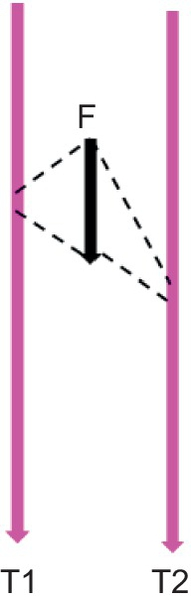
\includegraphics{sm_two_threads_same_function.jpg}
\end{center}
It is at this point that the stack properties play a role. The function body constructed by the compiler references all local addresses inside the function with the offset to an unknown stack pointer \textbf{SP}. Let \textbf{SP1} and \textbf{SP2} be the stack pointers of threads \textbf{T}1 and \textbf{T2}. The core running the thread \textbf{T1} (or \textbf{T2}) has a stack pointer register \textbf{SP} holding the value \textbf{SP1} (or \textbf{SP2}). When using a stack to manage local variables, switching the SP values switches a complete data set. The stack strategy to address local variables allows different threads to execute simultaneously the same function acting on different data sets.

\section{Memory System}
\subsection{Reading Data From Memory}
\begin{itemize}
	\item Current CPUs are load-store architectures in which data is always moved to core registers before being processed. Direct manipulation of memory locations does not occur in these architectures.
	\item The \textbf{L1} caches are rather small but fast memory blocks used both as \textbf{data caches}---to store the most recently accessed data---as well as \textbf{instruction caches}---to store the instructions to be executed by the core. Because they are partly used to store the instructions to be executed, the \textbf{L1} caches are never shared: threads running on different cores have their own, proprietary instruction stack. 
	\item The \textbf{L2} caches, instead, only store data, and they may be shared by several cores. In most systems, there is yet another cache level---called L3---between the L2 caches and the main memory.
\end{itemize}

\subsection{Writing Data To Memory}
When a data value is changed in a processor register, the CPU must proceed to update the original main memory location. Typically, the new data value is updated first in the \textbf{L2} cache, and from there on the network interconnect is activated to update the main memory. The following issues arise every time a new data value is updated in the \textbf{L2} cache:
\begin{itemize}
	\item First, the cache memory is no longer coherent with the main memory. How and when the main memory is updated is system dependent, but there is in most cases a time delay: the memory update is not atomic (instantaneous). Some systems choose to delay the writes in order to collect several data items in a write buffer, and then move them in a unique memory access in order to pay the big latency cost only once.
	\item Secondly, the updated cache memory is no longer coherent with other L2 caches in other sockets that may contain the old invalid value of the updated variable. The CPU that has performed the update must therefore inform all other CPUs engaged in the application that the relevant cache line is invalid, and that further reads of data in this cache line must get the data values from main memory. This is the cache \textbf{coherency issue}.
	\item Finally, because of the time delays in memory updates, those threads that must get updated data values from main memory must know, in one way or another, when the new updated values are available. They must make sure that, in performing a read, they recover the last updated value of the target data item. This is the \textbf{memory consistency issue}.
\end{itemize}

\end{document}          
